\subsection{Misura finale}\label{par:fondo2}

\subsubsection{Prese dati}

\begin{table}
	\centering
	\begin{tabular}{lllll}
		\toprule
		Data & Durata & Calibrazioni & Dati & Angolo \\
		\midrule
		19--20 feb    & 20 ore & dopo, solo \co & istogramma &           45.0\,\si{\degree} \\
		20--22 feb    & 40 ore & dopo           & istogramma &   61$\sfrac34$\,\si{\degree} \\
		26--27 feb    & 22 ore & prima e dopo   & campioni   &           15.0\,\si{\degree} \\
		27 feb \!--\! 1 mar & 38 ore & prima          & campioni   & \phantom{1}7.0\,\si{\degree} \\
		\bottomrule
	\end{tabular}
	\caption{\label{tab:misure}
	Prese dati per ricavare la massa dell'elettrone.}
\end{table}

Per ricavare la massa dell'elettrone usiamo quattro misure di spettro in coincidenza.
Tutte le misure durano circa 24 ore per avere sufficiente statistica (si è poi rivelata eccessiva).
Era nelle nostre intenzioni avere una calibrazione prima e dopo ogni misura
e avere l'elenco dei campioni anziché solo l'istogramma,
ma la rottura dell'alimentatore del crate ha ostacolato i nostri piani.
La misura dopo la quale il crate si è rotto ha la calibrazione solo prima;
due misure che abbiamo recuperato e che inizialmente erano solo misure di prova hanno la calibrazione solo dopo,
una delle quali non era intesa come misura di calibrazione e quindi ha solo il cobalto
(calibrazione 20feb in \autoref{tab:calibration}).
L'elenco delle misure è riportato in \autoref{tab:misure}.

\subsubsection{Funzione empirica spalla Compton}
\label{sec:empirical}

\begin{figure}
	\centering
	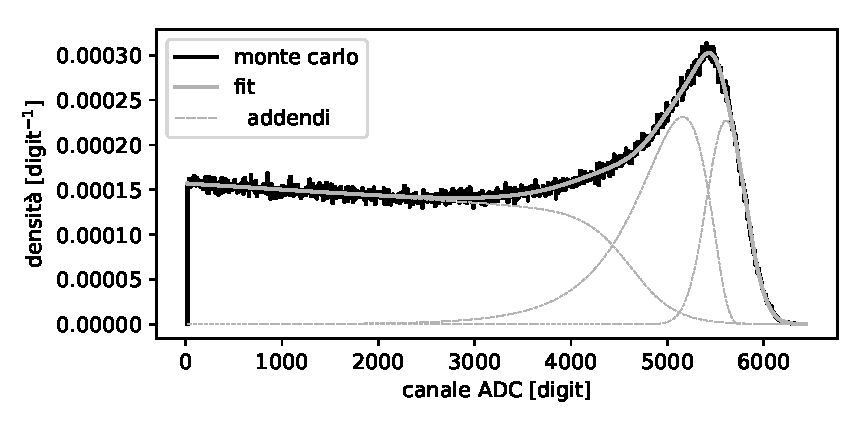
\includegraphics[width=33em]{empirical-secondary}
	\caption{\label{fig:empirical-secondary}
	Funzione empirica per descrivere la spalla Compton,
	ricavata con un fit della somma di una gaussiana, una log-gaussiana e la funzione di Fermi.
	Il Monte Carlo mostrato è ad angolo \SI{15}{\degree} e fotone della sorgente di \SI{1.33}{MeV}.}
\end{figure}

\begin{figure}
	\centering
	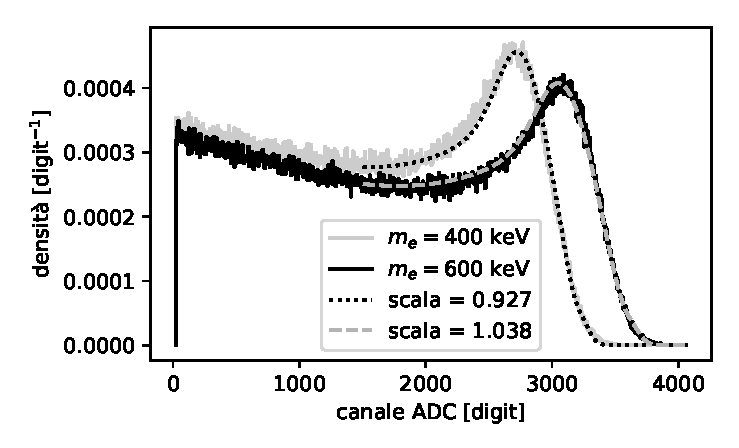
\includegraphics[width=28em]{empirical-test}
	\caption{\label{fig:empirical-test}
	Simulazione della spalla Compton a \SI{45}{\degree} e fotone della sorgente a \SI{1.33}{MeV}
	con diversi valori della massa dell'elettrone,
	fittata con la funzione empirica con solo un parametro di scala libero
	ed escludendo la parte sinistra della curva.}
\end{figure}

Per fare il fit della spalla Compton,
la simuliamo e fittiamo sulla simulazione una funzione empirica a 10 parametri
(vedi \autoref{fig:empirical-secondary});
per usarla sui dati blocchiamo tutti i parametri tranne un parametro di scala.
In \autoref{fig:empirical-test} verifichiamo che,
per valori della massa dell'elettrone di \SI{0.4}{MeV} e \SI{0.6}{MeV},
la funzione (ottenuta con massa \SI{0.511}{MeV}) descrive ancora sufficientemente bene la curva simulata.

\subsubsection{Fit degli spettri}

\begin{figure}
	\hspace{-8em}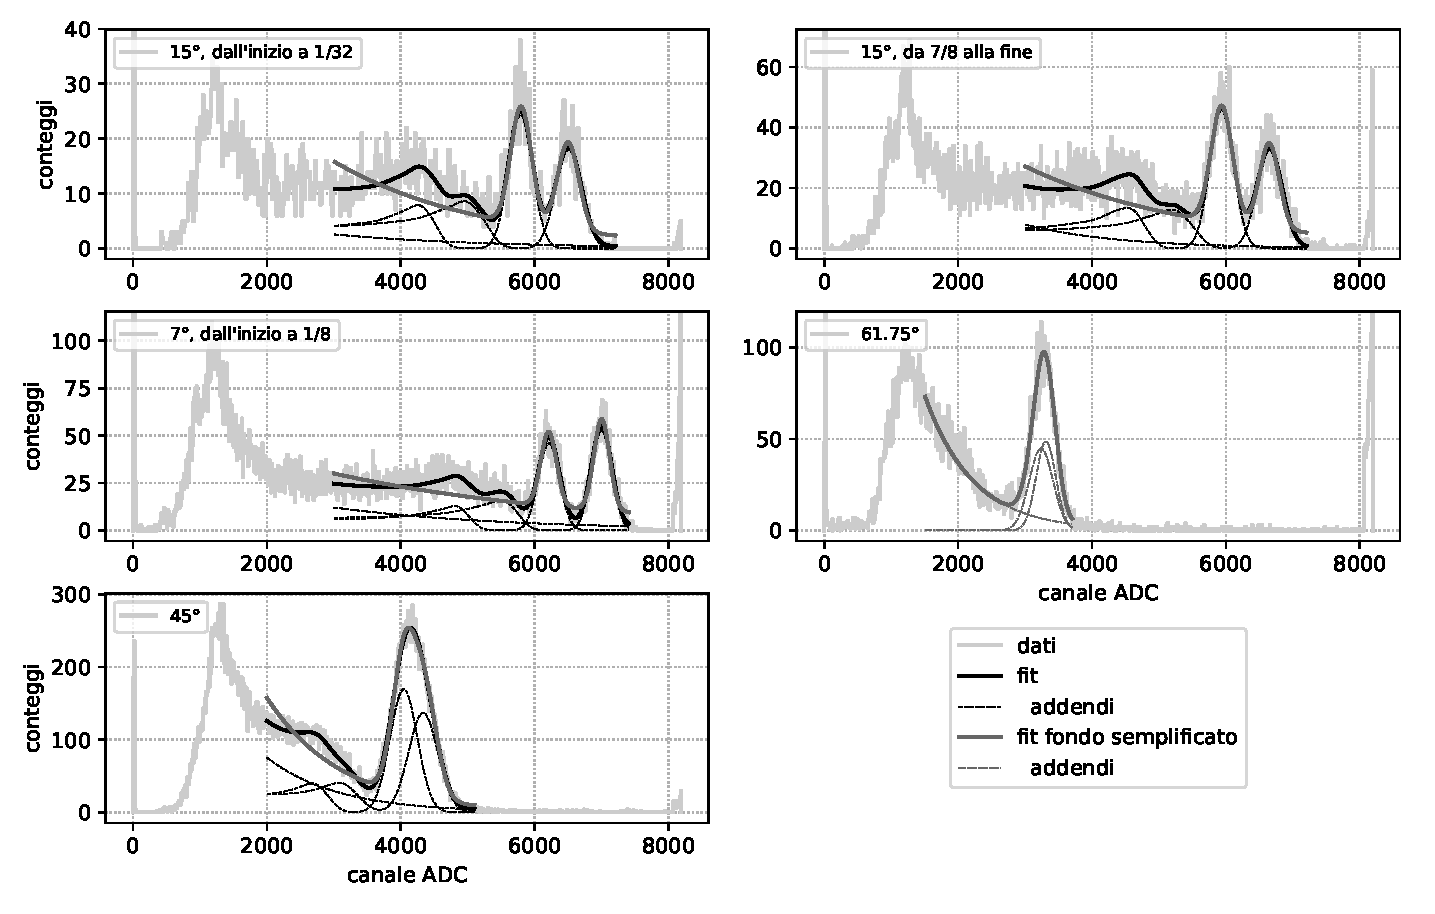
\includegraphics[height=0.9\textwidth]{fit}
	\caption{\label{fig:fit}
	Spettri del rilascio di energia nel NaI
	fittati con la somma di due gaussiane, due spalle Compton e un'esponenziale,
	oppure solo con due gaussiane e un'esponenziale (<<fondo semplificato>>).
	La presa dati a \SI{61}{\degree} è fittata solo con il fondo semplificato
	perché il fit completo è instabile.
	Nelle legende è eventualmente riportata
	la frazione temporale usata della presa dati.}
\end{figure}

Fittiamo ogni spettro con la somma di due gaussiane,
due spalle Compton espresse come in \autoref{sec:empirical}
e un'esponenziale.
Per verificare la dipendenza dal modello dei fondi
fittiamo anche senza spalle Compton, con solo l'esponenziale.
Quando i fotopicchi sono sovrapposti
fissiamo la normalizzazione relativa delle gaussiane a quella ottenuta dalla simulazione.
Imponiamo che il centro della gaussiana corrispondente al fotopicco a energia maggiore
sia maggiore del centro dell'altra.
Gli spettri e i fit sono riportati in \autoref{fig:fit}.

\subsubsection{Misura della massa}

\begin{figure}
	\hspace{-5em}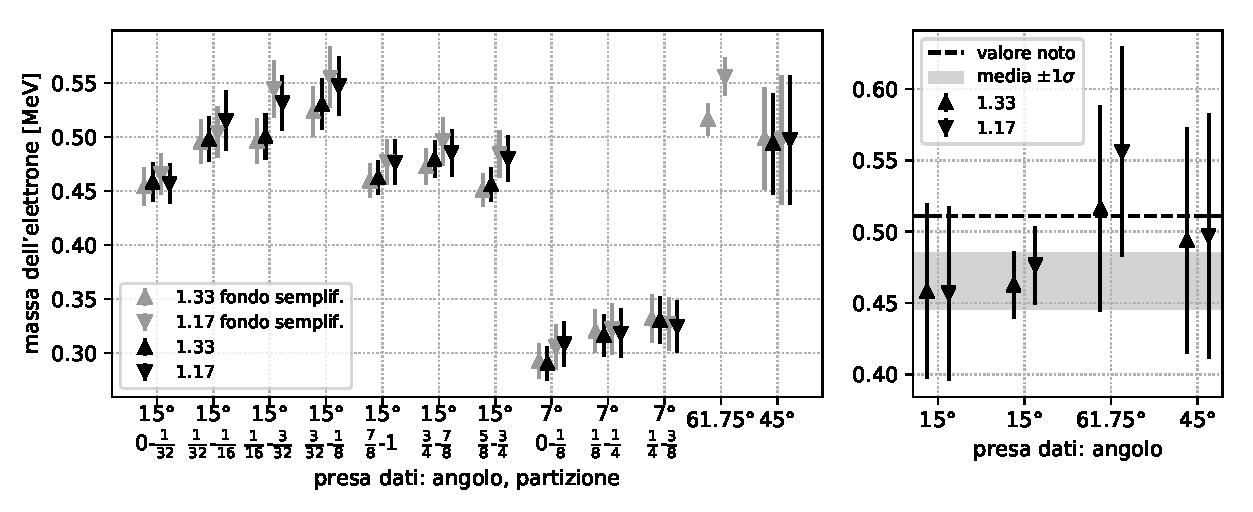
\includegraphics[width=46em]{me}
	\caption{\label{fig:me}
	Misure della massa dell'elettrone.
	Nel grafico a sinistra quelle ottenute da tutti i fit di spettri,
	anche nelle finestre temporali spostate usate per stimare l'incertezza di stabilità.
	Nel grafico a destra solo quelle usate per la media,
	con inclusa l'incertezza di stabilità nelle barre di errore.}
\end{figure}

Convertiamo i centri dei fotopicchi ottenuti dai fit degli spettri
da digit a MeV usando la calibrazione più vicina a ogni presa dati.
Per ogni fotopicco otteniamo la massa dell'elettrone invertendo la \eqref{energia_compton}.

\paragraph{Bias}

Per ogni fit, simuliamo i soli fotopicchi e li fittiamo con due gaussiane
per stimare il bias del fit. Calcoliamo direttamente il bias sulla massa dell'elettrone.
I~bias risultano circa \SI{-0.01}{MeV} per \SI{15}{\degree} e \SI{7}{\degree},
e dell'ordine di \SI{\pm0.001}{MeV} per \SI{45}{\degree} e \SI{61}{\degree}
(in cui la normalizzazione relativa delle gaussiane è imposta).
Sottraiamo i bias dalle masse calcolate.
Le masse sono riportate in \autoref{fig:me}.

\paragraph{Stabilità}

Per le prese dati di cui abbiamo i campioni anziché solo l'istogramma,
fittiamo lo spettro solo in una finestra temporale vicina alla calibrazione,
e ripetiamo il fit spostando la finestra.
Come incertezza sulla stabilità prendiamo la differenza
tra il risultato sulla finestra principale e sulla prima vicina,
prendendo la massima tra quella ottenuta con il fotopicco corrispondente a \SI{1.33}{MeV}
e quella del fotopicco \SI{1.17}{MeV}.

Quando abbiamo solo l'istogramma,
stimiamo l'incertezza di stabilità in questo modo:
dalla \eqref{eq:scalibur} si ottiene che la variazione relativa della massa misurata dell'elettrone
al variare della calibrazione è
\begin{equation}
	\label{eq:scal}
	r \is \frac{\Delta m_e}{m_e} = \frac1{E-E'}\left(\frac{\Delta E'}{E'}\right)E',
\end{equation}
dove $\Delta E'/E'$ è la variazione della scala di calibrazione.
Supponendo fissato $\Delta E'/E'$,
il rapporto tra le variazioni relative in due misure diverse $a$ e $b$ è
\begin{equation*}
	\frac{r_a}{r_b}
	= \frac{E - E'_b}{E - E'_a} \frac{E'_a}{E'_b}
	= \frac{1 - \cos\theta_b}{1 - \cos\theta_a}.
\end{equation*}
Se il tempo di acquisizione è diverso,
stimiamo la variazione della scala di $b$ come un random walk:
\begin{equation*}
	\left(\frac{\Delta E'}{E'}\right)_b = \left(\frac{\Delta E'}{E'}\right)_a \sqrt{\frac{t_b}{t_a}};
\end{equation*}
questa stima è conservativa perché l'effetto è integrato sul tempo.
Infine:
\begin{equation*}
	r_b = r_a \frac{1 - \cos\theta_a}{1 - \cos\theta_b} \sqrt{\frac{t_b}{t_a}}.
\end{equation*}
Nel nostro caso per $a$ prendiamo la presa dati a \SI{15}{\degree}
perché è quella con la maggiore incertezza di stabilità.

\paragraph{Misura a \SI{7}{\degree}}

Non usiamo la massa ottenuta dalla misura a \SI{7}{\degree}
perché risulta fortemente incompatibile con le altre misure.
Lo riteniamo plausibile perché, a questo angolo,
dalla \eqref{eq:scal} si ottiene che una variazione della scala dell'\SI1\%
provoca una variazione della massa misurata di \SI{0.26}{MeV},
\marginpar{In verità usando la formula mi viene che la scalibrazione
dovrebbe differire del \SI{15}\% tra 1.33 e 1.17,
cosa che non osservo in \autoref{fig:me}.}
quindi diventa molto significativo il tempo che intercorre tra la calibrazione
e l'inizio della presa dati.

\paragraph{Fondo semplificato}

Dalla \autoref{fig:me} si nota che i fit con fondo semplificato
non danno risultati significativamente diversi da quelli completi.
Inoltre, come si vede in \autoref{fig:fit},
i fit semplificati sono intenzionalmente poco sensati.
Fa eccezione la misura a \SI{61}{\degree}
in cui il fondo è effettivamente descritto dal modello semplificato.
Quindi per le misure useremo il fit completo,
tranne per quella a \SI{61}{\degree} in cui usiamo quello semplificato.

\paragraph{Media delle misure}

\begin{table}
	\centering
	\begin{tabular}{cccc|cccc}
		\toprule
		\multicolumn{4}{c|}{$E=\SI{1.33}{MeV}$} & \multicolumn{4}{c}{$E=\SI{1.17}{MeV}$} \\
		$\SI{15}{\degree}_\text{inizio}$ & $\SI{15}{\degree}_\text{fine}$ & \SI{61}{\degree} & \SI{45}{\degree} & $\SI{15}{\degree}_\text{inizio}$ & $\SI{15}{\degree}_\text{fine}$ & \SI{61}{\degree} & \SI{45}{\degree} \\
		\midrule
	   0.46(6) &     0.4\,\%  &   0.1\,\% &    0.1\,\% &   98.4\,\% &     0.3\,\% &   0.1\,\% &   0.0\,\% \\
	           & 0.463(23)  &   0.2\,\% &    0.1\,\% &    0.4\,\% &    91.5\,\% &   0.2\,\% &   0.1\,\% \\
	           &            & 0.52(4) &    0.0\,\% &    0.1\,\% &     0.2\,\% &  86.2\,\% &   0.0\,\% \\
	           &            &         &  0.49(6) &    0.1\,\% &     0.1\,\% &   0.0\,\% &  99.2\,\% \\
	           &            &         &          &  0.46(6) &     0.3\,\% &   0.1\,\% &   0.0\,\% \\
	           &            &         &          &          & 0.477(27) &   0.1\,\% &   0.1\,\% \\
	           &            &         &          &          &           & 0.56(4) &   0.0\,\% \\
	           &            &         &          &          &           &         & 0.50(7) \\
		\bottomrule
	\end{tabular}
	\caption{\label{tab:cov}
	Misure di massa (in \si{MeV}) usate per la media finale con la matrice di correlazione.}
\end{table}

Calcoliamo la media pesata con la matrice di covarianza delle varie misure di massa.
Calcoliamo anche separatamente le medie per le masse corrispondenti a $E=\SI{1.33}{MeV}$ e $E=\SI{1.17}{MeV}$.
Le masse usate per la media sono riportate in \autoref{tab:cov} e graficamente in \autoref{fig:me}.
Otteniamo (in \si{MeV}):
\begin{align*}
	m_e^{(1.33)}                &= \num{0.478 \pm 0.018}  ,    \\
	m_e^{(1.17)}                &= \num{0.497 \pm 0.020}  ,    \\
	m_e^{(1.17)} - m_e^{(1.33)} &= \num{0.019 \pm 0.008}  \quad(2.3\,\sigma),   \\
	m_e                         &= \num{0.477 \pm 0.017} = \\
	                            &=      0.477 \pm 0.016^{(\text{sist})} \pm 0.004^{(\text{stat})} \\
										 &=      0.477 \pm 0.014^{(\text{stab})} \pm 0.007^{(\text{cal})} \pm 0.004^{(\text{stat})} \pm 0.004^{(\text{ang})}.
\end{align*}
Il $\chi^2$ della media pesata è 8.1, per 7 gradi di libertà.
La nostra misura dista $2\,\sigma$ dal valore noto \SI{0.511}{MeV}.
